\subsection*{Циклические группы}
\begin{definition}
  \textit{Группой} называется множество $G$ с операцией умножения, обладающей следующими свойствами:
  \begin{enumerate}
    \item $(ab)c = a(bc),~\forall\;a,b,c \in G$ (ассоциативность)
    \item $\exists e \in G \text{ (единица)}\!:~ ae=ea=e~\forall a \in G$
    \item $\forall a \in G~\exists a^{-1} \in G \text{ (обратный элемент)},~aa^{-1} = a^{-1}a = e$
  \end{enumerate}
\end{definition}
Группа называется \textit{абелевой} или \textit{коммутативной}, если $ab=ba,~\forall a,\;b \in G$.

В любой группе может быть определена степень элемента $g \in G$ с целыми показателями:
$$ g^k = 
\begin{cases}
  \underbrace{g \cdot g \ldots \ \cdot g}_k,& \text{если } k > 0 \\
  e,& \text{если } k = 0 \\
  \underbrace{g^{-1} \cdot g^{-1} \ldots \ \cdot g^{-1}}_k,& \text{если } k < 0 \\
\end{cases}, ~~~k \in \Zint
$$
\begin{definition}
  Степени элемента $g$ образуют подгруппу группы $G$. Она называется \textit{циклической} и обозначается $<\!g\!>$
\end{definition}
\begin{definition}
  Наименьшее из натуральных $m$ для которого выполняется $g^m = e$ называется \textit{порядком} элемента.

  Если $m$ не существует, то порядок $g$ равен $+\infty$.

  Обозначение: $ord\;g = m$.
\end{definition}
\begin{theorem}
  Если $ord\;g = n$, то 
  \begin{enumerate}
    \item $g^m = e \Leftrightarrow n \mid m$
    \item $g^k = g^l \Leftrightarrow k \equiv l (mod\; n)$ 
  \end{enumerate}
\end{theorem}
\begin{Proof}
  \begin{enumerate}
  
    \item $m = np + r,~ r < n$

  $g^m = g^{np} \cdot g^r = (\underbrace{g^n}_{e})^p \cdot g^r = g^r$

  $\Rightarrow ~ g^m = e \implies g^r = e \implies r = 0 \implies n \mid m$

  $\Leftarrow$ так как $n \mid m$, то $r = 0  \implies g^r = g^0 = e$.
  \item $g^k = g^l \implies g^{k - l} = e$
  
  $\implies$ по первому утверждению $(k - l)\;\vdots \;n \implies k \equiv l$  (mod $m$)
\end{enumerate}
\end{Proof}

В аддитивной группе говорят не о степенях элемента $g$, а о его кратных. Обозначение: $m\;g$

Порядком элемента $g$ в \textit{аддитивной} группе называют наименьшее из натуральных $m$, такое, что $\underbrace{g+g+\ldots+g}_m = 0$(если $m$ существует).
\begin{theorem}
  Если $ord\;g = n$, то $ord\;g^k = \frac{n}{(n,k)},~(n,k) = \gcd(n,k)$ (НОД($n,k$))
\end{theorem}
\begin{Proof}
  Пусть $ord\;g^k = m$ и $(n,k) = d$. Тогда $n = n_1d,~ k = k_1d, ~(n_1,k_1) =1$.

  Так как $ord\;g = n$, то $g^n = e$. Также $(g^k)^m = e \implies km\;\vdots\;n \implies k_1dm\;\vdots \; n_1d \implies k_1m \;\vdots\; n_1$
  
  Так как $(k_1,n_1) = 1 \implies m\;\vdots\;n_1 \implies m = pn_1 = \frac{pn_1d}{d} = \frac{pn}{d}$ Так как $m = ord\; g^k$, то есть наименьшее натуральное число, удовлетворяющее определению порядка, $\implies p = 1$.

  $\implies ord\;g^k = m = \frac{n}{d} = \frac{n}{(n,k)}$.
\end{Proof}

\begin{definition}
  Группа $G$ называется \textit{циклической}, если существует такой элемент степени которого образует группу $G$. 
  
  $G = <\!g\!>$ и такой элемент называется \textit{образующим}.
\end{definition}

\begin{example}
  $\Zint$ аддитивная группа целых чисел является циклической с образующим элементом $1$ или $-1$

  $Z_n$ "--- циклическая группа с образующим элементом $[1]$.
\end{example}

\begin{definition}
  Число элементов конечной группы называется её \textit{порядком}.

  Обозначение: $\mathopen|G\mathclose|$
\end{definition}
\begin{example}
  Всякая бесконечная циклическая группа изоморфна группе целых чисел:

  $f: \Zint \to G$,

  $f: k \to g^k$.

  Всякая конечная цилкическая группа порядка $n$ изоморфна группе $Z_n$:

  $f: Z_n \to G$.

  
\end{example}
\begin{theorem}
  Всякая подгруппа циклической группы является циклической. 
  
\end{theorem}

\begin{theorem}
  В циклической группе порядка $n$ порядок любой подгруппы делит $n$ и для любого делителя $p$ числа $n$ существует одна подгруппа порядка $p$.
\end{theorem}

\subsection*{Разбиение на смежные классы}

\begin{definition}
  Пусть $G$ "--- группа, $H$ "--- подгруппа группы $G$. Элементы $g_1,\; g_2 \in G$ сравнимы по модулю $H$ $(g_1 \equiv g_2~(mod\;H))$, если $g_1^{-1}g_2 \in H$.

  $g_1^{-1}g_2 = h\in H \implies g_2 = g_1h$
\end{definition}

Отношение сравнимости по модулю $H$ является отношением эквивалентности:
\begin{enumerate}
  \item \begin{gather*}
    g_1 \equiv g_1~(mod\;H)\\
    (g_1^{-1}g_1) = e \in H
  \end{gather*}
  \item \begin{gather*}
    g_1 \equiv g_2~(mod\;H) \implies g_2 \equiv g_1~(mod\;H)\\
    g_1^{-1}g_2 \in H \implies (g_1^{-1}g_2)^{-1} \in H, \text{так как является обратным}.\\
    \implies (g_2^{-1}g_1 \in H) \implies g_2 \equiv g_1~(mod\;H).
  \end{gather*}
  \item \begin{gather*}
    g_1 \equiv g_2~(mod\;H) \wedge g_2 \equiv g_3~(mod\;H)\\
    \implies g_1 \equiv g_3~(mod\;H)\\
    g_1^{-1}g_2 \in H,~ g_2^{-1}g_3 \in H\\
    \implies (g_1^{-1}\underbrace{g_2)\cdot (g_2^{-1}}_{e} g_3) \in H \implies g_1^{-1}g_3 \in H\\
    \implies g_1\equiv g_3~(mod\;H).
  \end{gather*}
\end{enumerate}

\begin{figure}[H]
  \centering
  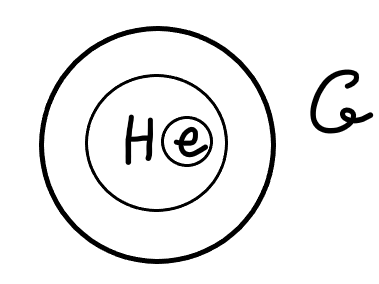
\includegraphics[height = 3cm]{images/groups_module.png}
  \caption{Пример}
\end{figure}

\begin{definition}
  Классы этой эквивалентности называются \textit{левыми смежными классами} группы $G$ подгруппы $H$.

  Смежный класс, содержащий элемент $g$, имеет вид $gH = \{gh,~h \in H\}$
\end{definition}

Одним из смежных классов является сама подгруппа $H$.

Если вместо $g_1^{-1}g_2\in H$ взять $g_2\,g_1^{-1}\in H$, то получим другое отношение эквивалентности. Классы этой эквивалентности называются \textit{правыми смежными классами}.
\begin{example}
  Смежные классы аддитивной группы $\Complex$ на подгруппе $\Real$ изображаются на комплексной плоскости прямой параллельной оси $Ox$

  $g + \Real,~g\in \Complex$

  $g + \Real = \{g + \lambda,~\lambda \in \Real\}$
  \begin{figure}[H]
    \centering
    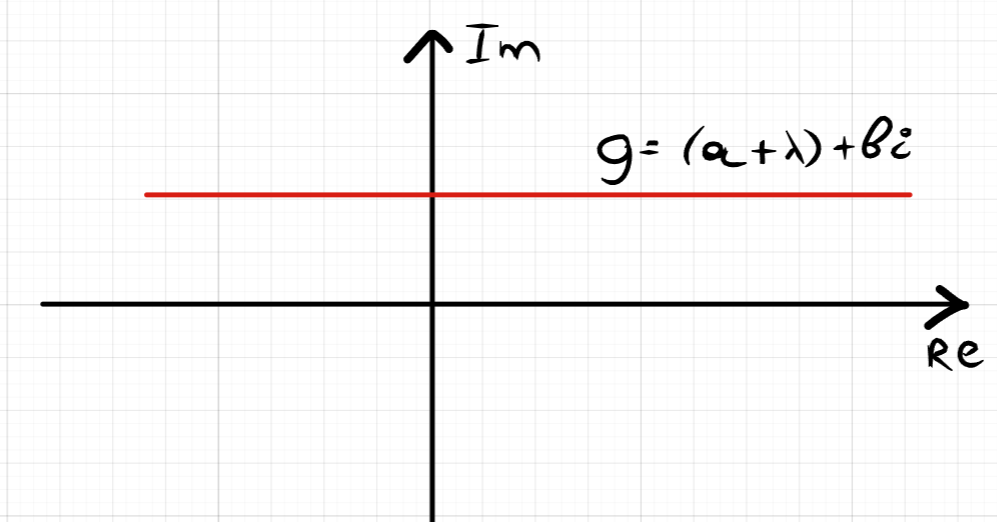
\includegraphics[height = 3cm]{images/groups_complex_example.png}
  \end{figure}
\end{example}
\begin{example}
  Смежные классы мультипликативной групп $\Complex^\ast = \Complex \setminus \{0\}$ по подгруппе $\Real^\ast_+$ изображаются на комплексной плоскости лучами, исходящими из начала координат.

  $g\Real^\ast_+ = \{g\lambda,~\lambda \in \Real\}$
  \begin{figure}[H]
    \centering
    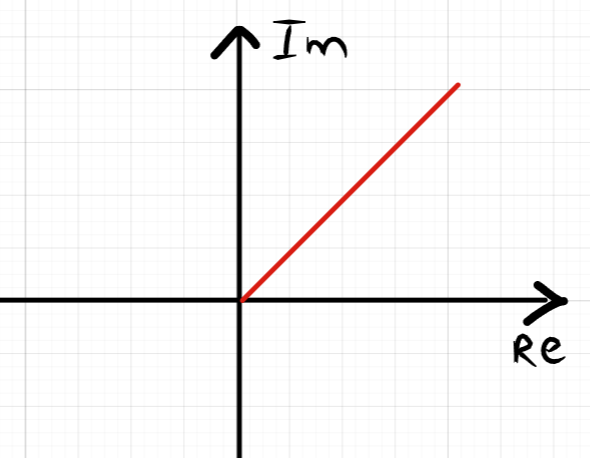
\includegraphics[height = 3cm]{images/groups_complex_withoutZero.png}
  \end{figure}
\end{example}

Множество левых смежных классов группы $G$ подгруппы $H$ обозначается $G/H$.
\begin{definition}
  Число смежных классов, если оно конечно, называется \textit{индексом} подгруппы $H$ и обозначается $\mathopen|G:H\mathclose|$.
\end{definition}
\begin{theorem}[Лагранжа]
  Если $G$ конечная группа, $H$ любая её подгруппа, то $\mathopen|G\mathclose| = \mathopen|G:H\mathclose| \cdot \mathopen|H\mathclose|$.
\end{theorem}

\begin{Proof}
  Все смежные классы $gH$ содержат одно и то же количество элементов равное $\mathopen|H\mathclose|$. Так как эти классы образуют разбиение группы $G$, то порядок группы $G$ равен произведению их числа на количество элементов подгруппы $H$ $\implies \mathopen|G\mathclose| = \mathopen|G:H\mathclose| \cdot \mathopen|H\mathclose|$.
\end{Proof}

\begin{definition}
  Подгруппа $H$ группы $G$ называется \textit{нормальной}, если $gH=Hg$, то есть $\forall g \in G:~ gHg^{-1} = H$ или $\forall g \in G, ~ \forall h \in H: ~ g \cdot h \cdot g^{-1} \in H$.

  Обозначение: $H \lhd G$, $G \rhd H$.
\end{definition}
В случае, если $H$ "--- нормальная  подгруппа группы $G$, то $G / H$ называется \textit{факторгруппой}.
$eH$ "--- единица этой группы.

\begin{definition}
  $f:~ G_1 \to G_2$ называется \textit{гомоморфизмом}, если $f(ab) = f(a)f(b),~ a,\,b \in G_1$.
\end{definition}
Свойства:
\begin{enumerate}
  \item $f(e) = e$
  \item $f(g^{-1}) = f(g)^{-1}$
  \begin{Proof}
    $f(a^{-1})f(a) = f(a^{-1}a) = f(e) = e \implies f(a^{-1}) = f(a)^{-1}$.
  \end{Proof}
  \item $Im\;f = \{f(a),~ a \in G_1\}$ "--- образ гомоморфизма. $Im\;f\subset G_2$.
  \item $Ker\;f = \{a \in G_1,~ f(a) = e\}$ "--- ядро.
  
  $Ker\;f$ есть нормальная подгруппа группа $G_1$.
  \begin{Proof}
    $a,\, b \in Ker\;f$

    $f(ab) = f(a) \cdot f(b) = e \cdot e = e \implies ab \in Ker\; f$

    $a \in Ker\; \implies f(a^{-1}) = e^{-1} = e \implies a^{-1} \in Ker\;f \implies Ker f\; \subset G_1$.

    $\forall g \in G_1,~a \in Ker\; f,~ g\,a\,g^{-1} \stackrel{?}{\in} Ker\;f$.

    $f(g\,a\,g^{-1}) = f(g)\cdot f(a)\cdot f(g^{-1}) = f(g)\cdot e \cdot f(g^{-1}) = f(g)f(g^{-1}) = f(g)(f(g))^{-1}= e$
    
    $\implies g\,a\,g^{-1} \in Ker\;f \implies Ker\; f$ есть нормальная подгруппа $G_1$.
  \end{Proof}
  \item $f(g_1) = f(g_2) \implies g_1 \equiv g_2 (mod\; Ker\;f)$
  \begin{Proof}
    $f(g_1) = f(g_2) ~/ \cdot f(g_1^{-1})$

    $f(g_1^{-1}) f(g_1) = f(g_1^{-1})f(g_2)$

    $e = f(g_1^{-1}g_2) \implies g_1^{-1}\,g_2 \in Ker\;f \implies g_1 \equiv g_2 (mod\; Ker\;f)$
  \end{Proof}
  \item $f(a^n) = (f(a))^n$
  \item $f:~ G_1 \to G_2$
  
  $\forall g \in G_1$ порядок элемента $f(g)$ делит порядок $g$.
  \begin{Proof}
    Пусть $ord\; g = k \implies g^k = e$

    $f(g^k) =  (f(g))^k \implies (f(g))^k = e \implies ord\;f(g) = k$.
  \end{Proof}
\end{enumerate}